\providecommand{\main}{../../../..}
\documentclass[\main/dresen_thesis.tex]{subfiles}
\renewcommand{\thisPath}{\main/chapters/theoreticalBackground/scattering/reflectometry}
\begin{document}
  \subsection{Reflectometry}
    \label{sec:theoreticalBackground:scattering:reflectometry}
    \label{ch:appendix:numericalMethods:parrat}
    \begin{figure}
      \centering
      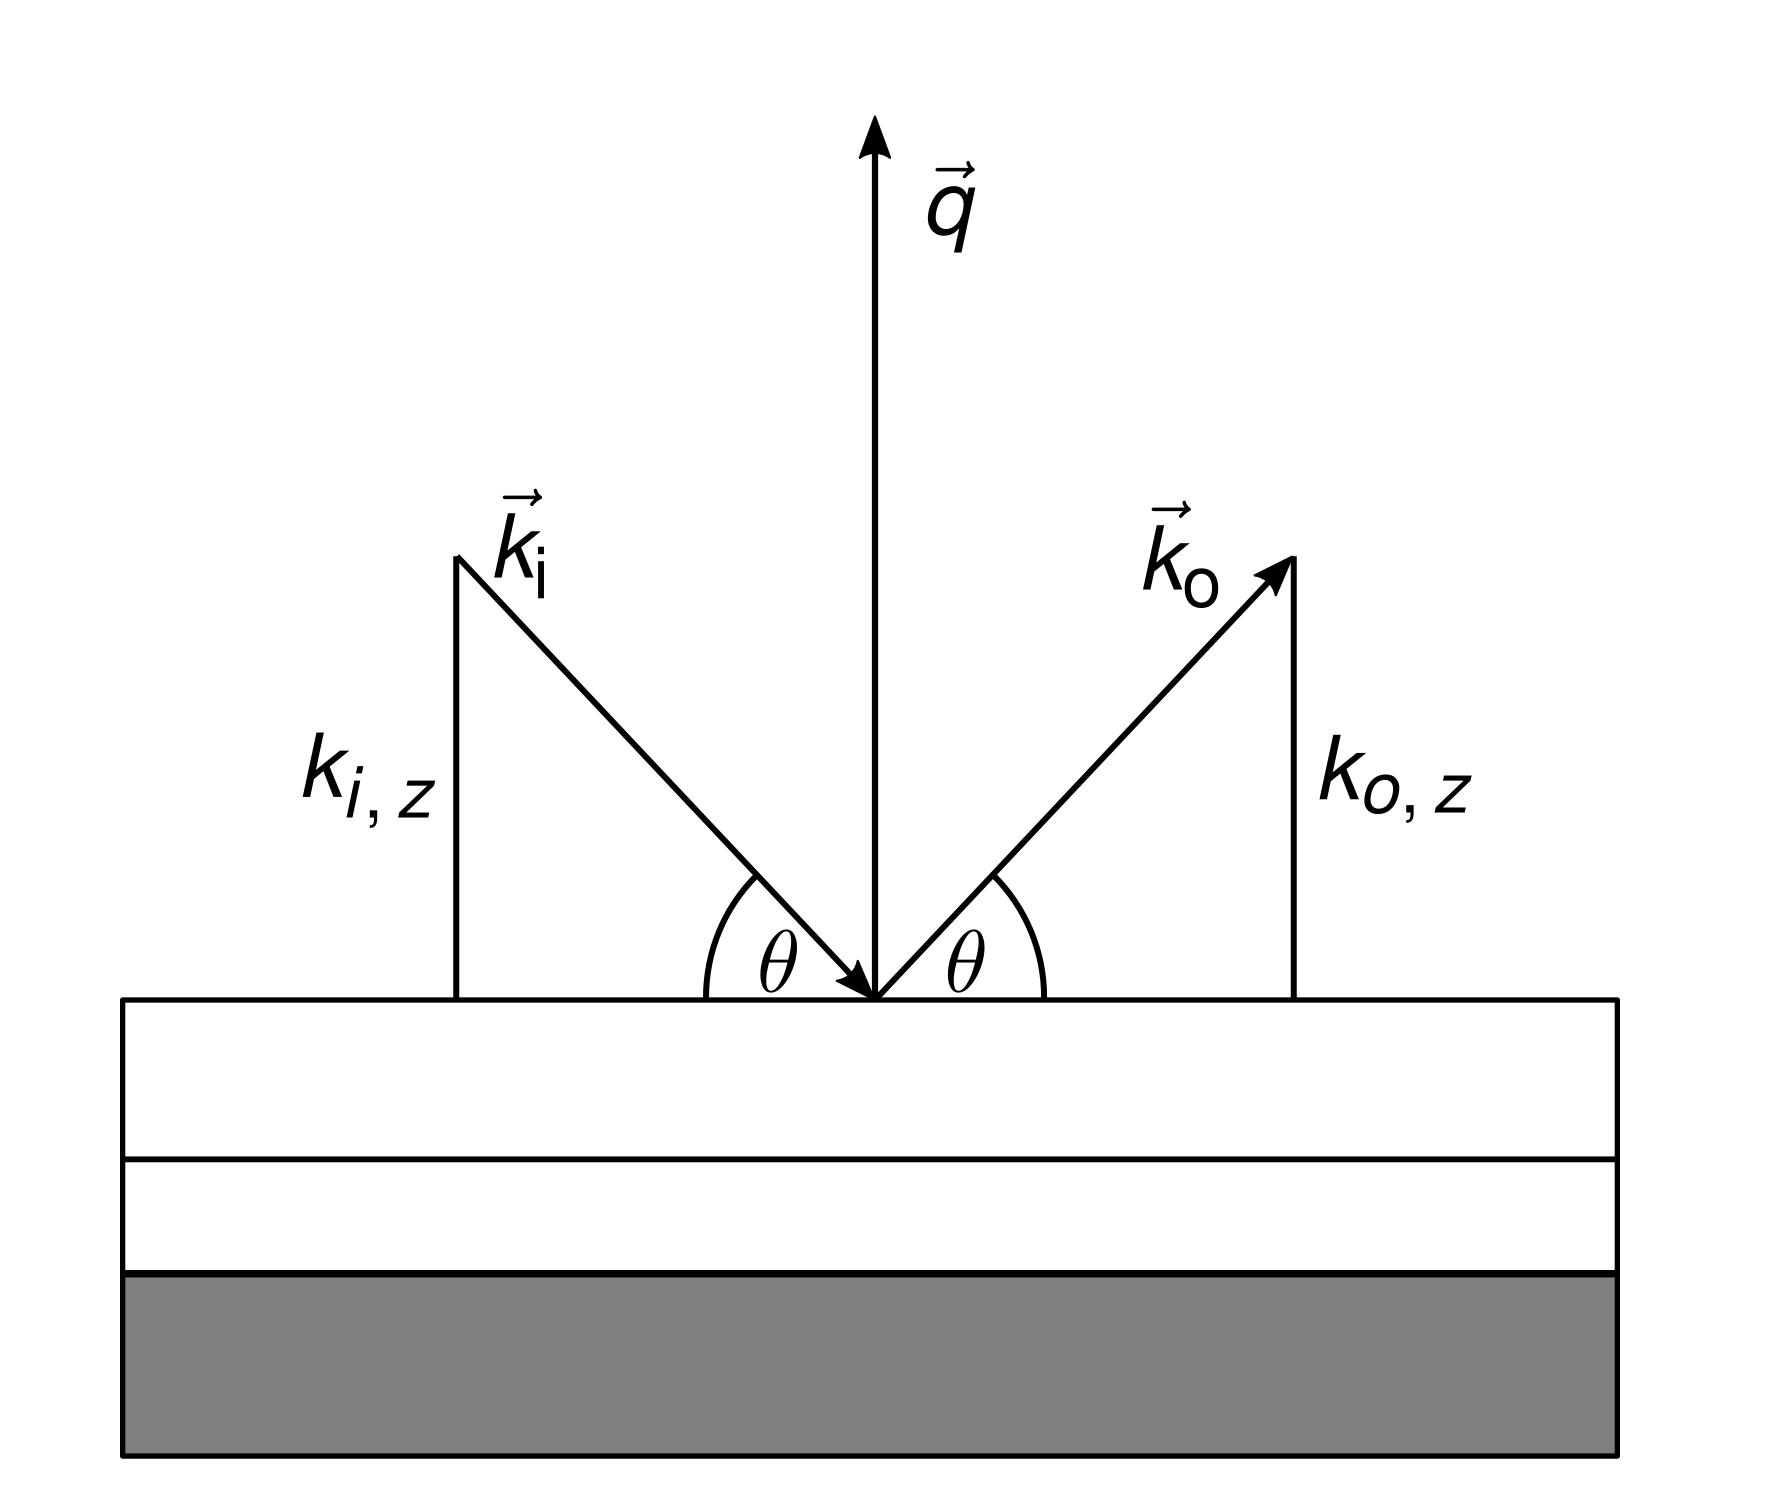
\includegraphics{scatteringTheory_reflectometryGeometry}
      \caption{\label{fig:theoreticalBackground:scattering:reflectometry:geometry}Geometry of a reflectometry experiment. The specular reflection  is measured and the reflectivity is then studied with respect to $q$.}
    \end{figure}
    A technique to study the vertical structure of a thin sample on a substrate is reflectometry.
    Here, the scattered intensity is measured under specular condition, whereby the scattering vector is parallel to the $\mathit{z}$-axis.
    In the previously discussed Born approximation of \refeq{eq:theoreticalBackground:scattering:scatteringTheory:differentialCrossSectionIntegralOverPotential}, this has the effect that the integral over the scattering potential reduces to a one dimensional problem
    \begin{align}
      \int \dint \vec{r} e^{-i\vec{q} \cdot \vec{r}} V (\vec{r}) \eq \int \dint z e^{-i q_z z} \bar{V} (z),
    \end{align}
    where $\bar{V}$ is the laterally integrated potential
    \begin{align}
      \bar{V}(z) \eq \int \dint x \int \dint y V(\vec{r}).
    \end{align}
    This motivates to discuss reflectometry as a one dimensional problem, where the sample is completely modeled by the laterally averaged scattering potential with respect to the vertical axis.
    And indeed, the scattering problem can be even solved exactly beyond the first Born approximation numerically efficient by Parratt's algorithm to account for multiple reflections on internal interfaces, total external reflection and refraction.

    We present Parratt's algorithm starting from the Schr\"odinger equation for neutrons, where the analogue derivation can be performed for X-rays from Maxwell's equations \cite{Daillant_1999_Xraya}.
    The Hamiltonian of the one dimensional Schr\"odinger equation for a neutron in a locally varying potential is given by
    \begin{align}
      H \eq \frac{\hbar^2 k_z^2}{2m_n} + \frac{2 \pi \hbar^2}{m_n} \mathrm{SLD}(z),
    \end{align}
    where $\mathrm{SLD}(z)$ is the laterally averaged SLD of the scattering nuclei in the studied thin film at height $z$.
    The sample is considered to be semi-infinite, meaning for $z \rightarrow -\infty$ the SLD has the value of the substrate and at a finite height $z > z_0$ it vanishes to zero.

    Using that the energy is given by the wave vector of the incoming neutron $k_{i,\,z}$ outside the material for elastic scattering, the Schr\"odinger equation writes as an equation that determines the wave vector of the neutron inside the sample at height $z$
    \begin{align}
      k_z^2 \eq   k_{i,\,z}^2 - 4 \pi  \mathrm{SLD}(z).
    \end{align}
    $k_{z,\,\mathrm{in}}$ relates to the scattering vector magnitude in reflectometry geometry by the simple relation $q \eq 2 k_{i,\,z}$.
    Thus by variation of $q$, the length scales of the wave vectors are tuned for the given SLD.
    For small $q$ the wave vector inside the medium becomes purely imaginary, which is the case for
    \begin{align}
      q_c \, < \, \sqrt{16 \pi \mathrm{SLD}},
    \end{align}
    and total external reflection occurs.
    Below this scattering vector all neutrons are reflected and a plateau is observed.
    Above this critical value, the reflectivity decreases rapidly, where the course of the curve allows to deduce on the internal structure of the sample.

    For numerical determination of the reflectivity, any potential can be discretized to a slab model, where each slab has a thickness $d_i$, a scattering length density $\mathrm{SLD}_i$ and a surface roughness $\sigma_{i,i+1}$ as parameter.
    Parratt's algorithm essentially steps iteratively from the substrate of the sample up to the surface and calculates the total reflectivity amplitude by summing the contribution of all paths the neutron can take to reflect.

    Starting at a model that only consist of a substrate, the problem is equivalent to that of the introductory quantum mechanics problem of a step potential, where the amplitudes for reflection and transmission between two layers with wave vector $k_i$ and $k_j$ are derived as the Fresnel equations
    \begin{align}
      r_{ij} \eq \frac{k_i - k_j}{k_i+k_j},\\
      t_{ij} \eq \frac{2 \sqrt{k_i k_j}}{k_i+k_j},
    \end{align}
    where the indices mean that the neutron is incoming from layer $i$ and reflects on/transmits to layer $j$.
    When a layer is added on top of the substrate, the path of the neutron is now either to reflect directly at the layer surface with $r_{21}$ or it can transmit into the sample and take one of the many other possible paths as depicted in \reffig{fig:theoreticalBackground:scattering:reflectometry:parratt}, which can include multiple transmissions and reflections before it exits the sample and contributes to the total reflection amplitude.
    \begin{figure}
      \centering
      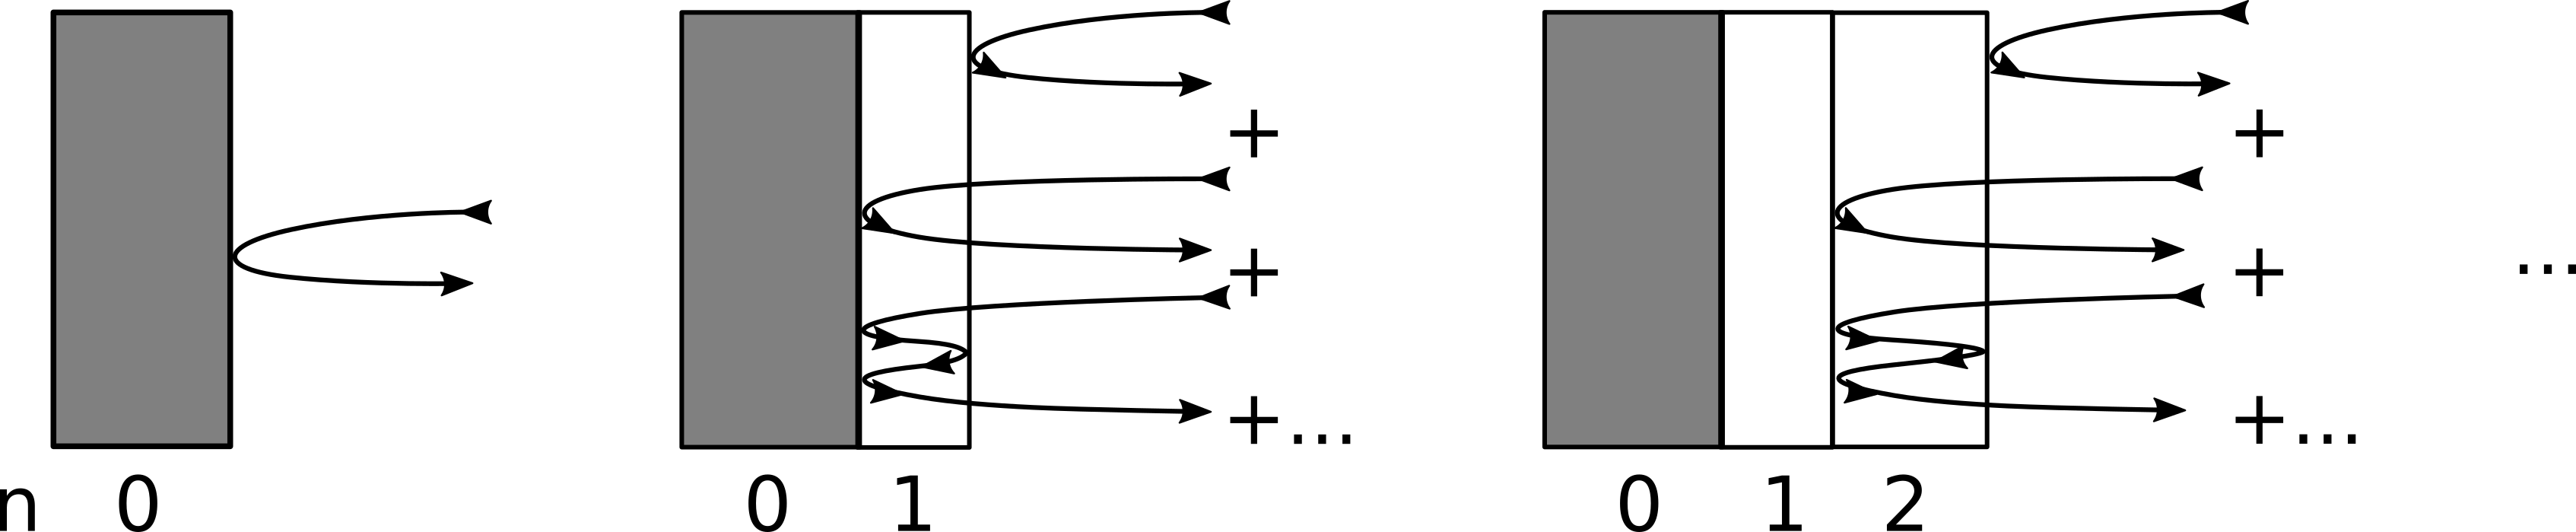
\includegraphics{scatteringTheory_parrattsAlgorithm}
      \caption{\label{fig:theoreticalBackground:scattering:reflectometry:parratt}Depiction of Parratt's algorithm: Starting from a the substrate, all possible paths that contribute to the reflectometry are summed iteratively, where the reflictivity of  to obtain the reflectivity of the slab model.}
    \end{figure}
    When adding all possible paths, for each distance the neutron travels within the material, a picked up phase $e^{i k_i d_i}$ has to be considered.
    The sum of all paths can then be summed as geometric sum, as can be seen by
    \begin{align}
      \begin{split}
        r &\eq r_{21} + t_{21} r_{10} t_{12} e^{2 i k_1 d_1} + t_{21} r_{10} r_{12} r_{10} t_{12} e^{4 i k_1 d_1} + \ldots\\
        &\eq r_{21} + t_{21} t_{12} r_{10} e^{2 i k_1 d_1} \sum_{n\eq0}^\infty \biggl(r_{12} r_{10} e^{2 i k_1 d_1}\biggr)^n\\
        &\eq r_{21} + \frac{t_{21} t_{12} r_{10} e^{2 i k_1 d_1}} {1 - r_{12} r_{10} e^{2 i k_1 d_1}}\\
        &\eq \frac{r_{21} + r_{10} e^{2 i k_1 d_1}} {1 + r_{21} r_{10} e^{2 i k_1 d_1}},
      \end{split}
    \end{align}
    where in the last step it is used that $r_{ij} \eq -r_{ji}$, $t_{ij} \eq t_{ji}$ and $r_{ij}^2 + t_{ij}^2 \eq 1$.
    This reflection amplitude contains all possible path the neutron can take once transmit into layer $1$ to return to layer $2$.
    When another layer is added on top, the problem therefore repeats itself, when this reflection amplitude is used instead of the substrate reflection amplitude.

    Thus, Parratt's formula consist of iteratively applying the formula
    \begin{align}
      r_{i} \eq \frac{r_{i+1,i} + r_{i-1} e^{2 i k_i d_i}} {1 + r_{i+1,i} r_{i-1} e^{2 i k_i d_i}},
    \end{align}
    where $r_0$ is given for the substrate by the Fresnel equation as $r_{10}$.
    To include the surface roughness of the layers, the reflectometry amplitude of the Fresnel equation is modified by the Névot-Croce factor \cite{Nevot_1980_Carac}
    \begin{align}
      r_{ij} \eq \frac{k_i - k_j}{k_i+k_j} e^{-2 k_i k_j \sigma_i^2},\\
    \end{align}
    which can be shown to be equivalent to replacing the sharp step between two layers by a smooth error function of width $\sigma$ \cite{Tolan_1999_XRaySc}.
    Thereby, the roughness parameter in the Névot-Croce factor effectively models the interface by an ensemble of Gaussian distributed smooth surfaces around the mean value.

    After the reflectivity amplitude is calculated, the reflictivity of the model is given by the square of the absolute value $R \eq |r|^2$.
    By measuring the reflectivity over a $q$ range that is adequate for the length scales in the sample, the comparison of the data with models allows to deduce on the structure of the sample.
    The experimental techniques and details to obtain reflectivity curves for X-rays and neutrons is described in the section for experimental methods in \refch{ch:methods:xrr} and \refch{ch:methods:nr}, respectively.
    X-ray reflectometry allows to study the average electron density in a sample with depth resolution, whereas neutron reflectometry allows to probe the nuclear structure.
    Additionally, polarized neutron reflectometry (PNR) allows in principle to resolve the magnetic density with depth resolution.
\end{document}